\documentclass[a4paper,12pt]{book}
\usepackage[latin1]{inputenc}
\usepackage[spanish]{babel} 

\title {Visi�n por computador}
\author {Carlos Le�n \and Jorge Mendoza \and Diego S�nchez}

\begin{document}
\maketitle
\thanks {Gracias a Jos� Antonio L�pez por su ayuda con el robot, y a Juan Rodr�guez por su ayuda con Prolog.}
\part {Definici�n del proyecto}
\chapter {Descripci�n del proyecto}

\section{Introducci�n}

El proyecto consiste en un motor modular de visi�n no dependiente del entorno y el reconocimiento de mensajes, a trav�s de las im�genes capturadas, para la implantaci�n del sistema de �rdenes de un robot. Para la demostraci�n de la funcionalidad se usar�n un entorno en 3D y un robot construido desde cero.


\chapter{Gesti�n de configuraci�n}

\section{Introducci�n}

\chapter{Dise�o y arquitectura del proyecto}

\chapter{Dise�o y arquitectura del proyecto}

\section{Introducci�n}
En este cap�tulo vamos a dar una idea global y poco exhaustiva, pero concreta, de la arquitectura de \emph{Visi�n por Computador}. Tiene dos apartados importantes: la arquitectura modular, y la conexi�n de estos m�dulos.

\section {Arquitectura de la aplicaci�n. M�dulos en tuber�a}
Al dise�ar la aplicaci�n escogimos implementar un sistema altamente modular para conseguir un alto grado de independencia en el desarrollo y de facilidad de ampliaci�n. Por esta raz�n hemos invertido parte del trabajo en desarrollar una plataforma propia de enlace de m�dulos, en la que la una parte de la aplicaci�n (lo que hemos denominado {\em pipeline} o {\em tuber�a}), se encargue de realizar el trabajo mec�nico, que, b�sicamente, se compone de:
\begin{itemize}
\item Conectar los m�dulos mediante puertos independientes con diferente informaci�n por puerto, pudiendo crear conexiones {\em 1 a 1}, {\em n a 1}, {\em 1 a n}, y {\em n a n}.
\item Iniciar y cerrar los m�dulos, creando y liberando la memoria necesaria y llamando a las funciones pertinentes de cada m�dulo.
\item Gestionar un reloj de ciclos de ejecuci�n, transmitiendo la acci�n por el grafo que forma la arquitectura de m�dulos.
\item Control de proyectos de aplicaci�n din�micos, mediante definici�n de los mismos en {\bf XML}. De esta forma, diferentes archivos de configuraci�n de proyecto puden crear aplicaciones totalmente distintas sin tener que reprogramar nada.
\item Manejo de errores mediante retrollamadas a funciones definidas por el usuario.
\end{itemize}
El {\em pipeline} es multiplataforma y funciona con m�dulos compilados desde {\em cualquier lenguaje est�ndar} como bibliotecas din�micas. Esto dota a la aplicaci�n de un marco muy amplio de uso en cualquier �mbito de desarrollo.


\section{Diagrama de pipeline de ``Visi�n por Computador''}
En la figura \ref{diagrama_vision_computador} hemos esquematizado todo el proceso que siguen los datos de nuestra aplicaci�n hasta llegar a una salida visible por el usuario. Los datos comienzan en la interfaz de im�genes (puede ser una imagen de c�mara, un v�deo, una imagen fija...), y descienden por el grafo de m�dulos hasta el \textbf{robot} o el \textbf{entorno 3D}. Asimismo, tenemos tambi�n de entrada las ventanas de par�metros, que dotan a los filtros de los valores necesarios \emph{en tiempo real}.

Tras el filtrado pertinente de cada imagen, se las lleva a un m�dulo de proceso (redes neuronales para los guantes, y algoritmo de \emph{OCR} para el texto), y, paralelamente, a ventanas de visualizaci�n, para depuraci�n y comprobaci�n de resultados. Se filtran las se�ales err�neas y, para el m�dulo de texto, se env�a la informaci�n a un m�dulo de DCG\footnote{Definite clause grammar} que genera una salida como respuesta ``inteligente''. Cuando la informaci�n ya ha sido extra�da de cada imagen, s�lo queda unificarla con el resto de datos, para dar una salida coherente.
%\begin{figure}
%  \label{diagrama_vision_computador}
%  \centering

  %\includegraphics[width=120mm]{pipeline.eps}

  %\caption{Diagrama de tuber�a}
%\end{figure}

\begin{figure}
  \centering
  \includegraphics[width=13.608cm,height=11.404cm,bb=0 0 1113 854]{pipeline.eps}
  \caption{Diagrama de tuber�a}
  \label{diagrama_vision_computador}
\end{figure}





\chapter{Planificaci�n}

\part{Anexos}

\chapter{M�dulo de generaci�n de im�genes}

\section{Introducci�n}
Este m�dulo tiene como objetivo la creaci�n y modificaci�n de un b�fer de colores (una imagen en formato plano) para la alimentaci�n de la tuber�a de visi�n. Obtiene, de diferentes fuentes, imagenes codificadas de diferentes maneras, y genera, en un formato unificado, una imagen sin comprimir.

\section {Im�genes generadas}
% Hablar de los formatos

\section {Arquitectura y funcionamiento del m�dulo}
El m�dulo sigue las interfaces de comunicaci�n con el {\em pipeline}, de modo que crea los b�feres en la funci�n de iniciar, a la vez que, seg�n se haya instanciado a trav�s de la configuraci�n del XML que define el proyecto, abre la comunicaci�n con las bibliotecas pertinentes, en funci�n de los argumentos.

En el ciclo de im�genes se procede seg�n sea el funcionamiento. En el caso de que las im�genes cambien cada ciclo (no pasa cuando son im�genes de un color fijo o cargadas de archivo), se obtiene del recurso indicado el b�fer en el formato que ofrezca la biblioteca, y se transforma al formato de salida com�n, como se ha comentado en la secci�n anterior. Una vez que se ha hecho esto, se ``deposita'' en el puerto de salida la imagen resultante, habiendo ya dado uniformidad a las diferentes entradas, haciendo que el {\em pipeline} no dependa de las fuentes generadores de im�genes a m�s bajo nivel.

En la funci�n de cerrar simplemente libera los recursos.

\section {Bibliotecas}
Para la generaci�n resultados desde diferentes fuentes, el m�dulo hace uso de una serie de librer�as; son las siguientes:

\begin {itemize}
\item {\bf SANE}: Sane (Scanner Access Now Easy) es una biblioteca originariamente para interfaces con esc�neres, pero ampliada para cualquier dispositivo de im�genes. A trav�s de esta biblioteca accedemos a la c�mara.
\item {\bf Xine}: Xine-lib tiene como objetivo la reproducci�n de archivos de v�deo en varios formatos (los m�s usuales, tambi�n puede aceptar formatos nuevos a trav�s de {\em plugins}). A trav�s de Xine cargamos un v�deo en el m�dulo de im�genes y lo reproducimos.
\item {\bf Gdk}: Usamos Gdk para cargar f�cilmente archivos de im�genes, y usarlos as� como fuentes sencillas de im�gnenes cuyo resultado se conoce.
\item {\bf C�digo propio}: Tambi�n hemos implementado, para pruebas principalmente, las siguientes funcionalidades del m�dulo:
  \begin {itemize}
  \item {\bf Generaci�n de colores planos}: Pintamos todo el b�fer de un color. Es muy �til para comprobar el funcionamiento de los filtros.
  \item {\bf Generaci�n de im�genes aleatorias}: Rellena la matriz de colores con colores al azar, de esta manera vemos c�mo los filtros aceptan o dejan de aceptar los valores.
  \end {itemize}
\end {itemize}

\section {C�digo}
Ver anexo: documentaci�n del m�dulo de im�genes.c, en \ref {imagenes_8c} (p�gina \pageref{imagenes_8c}).

%%% Local Variables: 
%%% mode: latex
%%% TeX-master: "vision"
%%% End: 

\chapter{M�dulo de Entorno 3D}

\section{Introducci�n}

El entorno virtual 3d constituye un interface visual con el usuario que puede observar la simulaci�n de las evoluciones de un robot que se desplaza por un escenario siguiendo las �rdenes procesadas por el sistema de visi�n por computador.

Con esta aplicaci�n, es posible evaluar y testar las funcionalidades que se han implementado sin tener que llegar a la integraci�n del sistema en una entidad rob�tica real.

\section{Detalles} 
\begin{itemize} 
\item {\bf Entrada}: Una estructura de datos que contiene una cadena de �rdenes y otra de par�metros.  
\item {\bf Salida}: Movimiento del robot virtual.
\item {\bf Descripci�n}: M�dulo que a partir de unas �rdenes representa el desplazamiento de un robot virtual a trav�s de un escenario en tres dimensiones.
\end{itemize} 


\section{Especificaci�n}

Para cumplir con su cometido, la aplicaci�n debe poseer las siguientes caracter�sticas funcionales:

\subsection{Representaci�n tridimensional de un entorno/escenario}

Teniendo en cuenta que una de las principales motivaciones para elaborar un sistema de �rdenes mediante visi�n artificial es la de implementar un dispositivo de navegaci�n que permita a un aut�mata desplazarse por su entorno, es fundamental simular gr�ficamente un escenario sobre el cu�l el robot virtual pueda desenvolverse. Esta representaci�n debe ser lo m�s inmersiva posible para que la precisi�n de la simulaci�n sea adecuada.
\subsection{Representaci�n de un robot capaz de desplazarse por su entorno}

Debe existir una entidad (en este caso un modelo 3D) dentro de la simulaci�n que represente la ubicaci�n, orientaci�n y desplazamientos resultantes de las distintas �rdenes procesadas por el sistema de control. Aunque en principio no es relevante, se ha intentando que esta entidad cumpla con ciertos criterios de dise�o que empaticen con los sistemas motrices m�s comunes en aut�matas (uso de ruedas, orugas, etc).
\subsection{Sistema de control}

Las diferentes �rdenes que son procesadas por el sistema de visi�n artificial, son analizadas para establecer las nuevas propiedades de posicionamiento, direcci�n, etc de la entidad que representa al robot. Esta interacci�n se realiza mediante el paso de mensajes distribuidos por el pipe que se encarga de la interconexi�n entre los diferentes m�dulos. Adem�s, es necesario que de forma aut�noma la aplicaci�n pueda procesar diferentes comandos emitidos por el usuario mediante el teclado y rat�n para poder controlar otros aspectos secundarios de la simulaci�n, como son el posicionamiento de la c�mara, activaci�n de diferentes efectos gr�ficos, etc.
 
\subsection{Sistema de c�maras interactivas}

Para poder visualizar de forma �ptima todos los componentes de la simulaci�n, es necesario poseer un sistema de c�maras que permita seguir c�modamente las evoluciones del robot por el escenario, as� como permitir al usuario adaptar la posici�n de las distintas c�maras para obtener el �ngulo de visi�n m�s relevante en cada momento.

\section{Implementaci�n}

La consecuci�n de las especificaciones previamente expuestas se ha conseguido mediante la implementaci�n de un amplio conjunto de caracter�sticas relacionadas principalmente con la programaci�n gr�fica 3D. A continuaci�n se describen detalladamente:

\subsection{Uso de DirectX 9.0}

La implementaci�n de los gr�ficos tridimensionales se ha realizada sobre la librer�a gr�fica Direct3D incluida en DirectX 9.0. Se ha optado por este est�ndar en vez del uso tambi�n muy extendido de la librer�a OpenGl por razones acad�micas, en el sentido de que previamente hab�amos tenido experiencia con OpenGl en otros proyectos y esta se presentaba como una oportunidad id�nea para investigar nuevas tecnolog�as. Cabe se�alar que ambas librer�as poseen similar potencialidad por lo que la elecci�n por razones funcionales no era especialmente relevante.
\subsection{Modelos 3D creados sobre 3dStudio Max 6.0}

Se ha empleado la herramienta de modelado 3dStudio Max para la elaboraci�n de los modelos tridimensionales tanto del escenario como del robot. Para su posterior integraci�n con la aplicaci�n, se ha utilizado un conversor que compatibiliza el formato usado por 3dStudio con el usado por Direct3D (archivos .X). En cuanto al apartado de las texturas, se ha utilizado Adobe PhotoShop para su realizaci�n.
\subsection{Terreno generado a partir de un mapa de altura}

Como parte del escenario, se ha incluido un terreno que es generado de forma procedural a partir de un mapa de altura. Una vez calculado la malla 3D de dicho terreno, se genera de forma procedural  la textura a partir de diferentes im�genes que se interpolan siguiendo como criterio la altitud del terreno. De esta forma, seg�n lo alto o bajo que est� el terreno, este presentar� el aspecto de diferentes materiales ( hierba para las zonas bajas, roca en las cumbres de las monta�as, etc). Por �ltimo se utiliza un algoritmo primitivo de sombreado que ilumina la textura resultante de forma coherente respecto a la posici�n de la luz en el escenario ( en este caso del sol).

\subsection{Iluminaci�n din�mica}

Para otorgar una mayor sensaci�n de integraci�n de la entidad que se desplaza con  el escenario, se ha utilizado iluminaci�n din�mica. De esta forma el robot es iluminado correctamente seg�n su posici�n actual, incrementando adem�s el realismo en la percepci�n de los materiales al visualizarse efectos de brillo, luz difusa, variaci�n crom�tica,etc.

 
\subsection{Iluminaci�n est�tica. LightMaps}

Los elementos est�ticos del escenario no requieren de iluminaci�n din�mica ya que su posici�n no var�a durante la ejecuci�n de la aplicaci�n. Para ahorrar recursos, es habitual el uso de texturas secundarias tambi�n llamadas lightmaps que codifican la informaci�n sobre la iluminaci�n que ese objeto recibe. En este caso, se ha utilizado una �nica textura resultado de la fusi�n de la textura primaria y los lightmaps para optimizar el rendimiento.

 
\subsection{Sombreado Din�mico. Stencil Buffer}

De forma an�loga a la iluminaci�n din�mica, el sombreado din�mico es un efecto que permite la integraci�n de objetos m�viles en escenarios de forma muy realista. Se ha implementado un algoritmo de sombreado que se basa en el uso del Stencil Buffer. Este algoritmo es bastante costoso en cuanto a recursos de la tarjeta gr�fica, por lo que sueles implementarse para ser soportado por tarjetas con aceleraci�n 3D de �ltima generaci�n.

\subsection{Luces Glow. Lens Flares}

Las luces Glow son puntos lum�nicos que producen un haz a su alrededor cuando se mira directamente. En este caso, se ha implementado un punto de luz que representa al sol. Adem�s, se ha implementado un efecto conocido como Lens Flares que se produce cuando se enfoca un sistema �ptico (c�mara de fotos, de video,etc) sobre un foco de luz intensa. Este efecto produce  una serie de reflejos residuales que se ubican de forma relativa a la luz que los origina. Se ha introducido por razones est�ticas y para incrementar la inmersi�n en el entorno virtual.

\subsection{Sistema de c�maras}

Se han implementando varios sistemas de c�maras para ofrecer m�ltiples posibilidades al usuario de seguir la acci�n que se desarrolla en la simulaci�n. Se dividen en:

\begin{itemize}

\item C�mara de seguimiento r�gido: La c�mara se sit�a siempre detr�s del robot y sigue cada uno de sus movimientos permaneciendo siempre a una misma distancia.

\item C�mara de seguimiento orbital: A diferencia de la anterior, esta c�mara orbita alrededor del robot manteniendo siempre su punto de enfoque fijado en �l.

\item C�mara fija: Se establece una posici�n de la c�mara donde permanece fija mientras enfoca y sigue los movimientos del robot.

\item C�mara libre: Con esta c�mara se puede navegar por todo el escenario as� como enfocar a los puntos de mayor inter�s para el usuario.
\end {itemize}

\subsection{Sistemas de part�culas}

De forma gen�rica, se ha implementado un sistema de part�culas para poder introducir efectos especiales y atmosf�ricos como pueden ser humo, fuego, lluvia, nieve, etc. Los sistemas de part�culas combinan una representaci�n gr�fica mediante billboards( pol�gonos especiales que mantienen siempre su orientaci�n respecto a la c�mara) y un sistema de control f�sico que determina el comportamiento de las part�culas en cuanto a aceleraci�n, direcci�n, tiempo de vida, turbulencia, etc.

 
\section{Dise�o}

El dise�o de la aplicaci�n es bastante sencillo en cuanto a su estructura jer�rquica. Existe una clase que contiene a la VentanaPrincipal de la aplicaci�n y que constituye el n�cleo de la ejecuci�n. Esta clase contiene un objeto del tipo Escena que es el que administra el resto de entidades con sus correspondientes representaciones gr�ficas. As�, la escena es el contenedor para otros objetos como son el Terreno, el Cielo, SistemaPart�culas, C�mara, y el resto de entidades como el escenario y el propio robot que pertenecen a la clase Objeto. Respecto a esta �ltima clase, destacar que posee como atributo un objeto de la clase Mesh que constituye la representaci�n gr�fica de la entidad (es decir, la maya 3d). Para gestionar la carga de los diferentes modelos 3d, existe una clase est�tica llamada MeshManager que comprueba que no se carguen en memoria varios modelos del mismo tipo. Por tanto, la creaci�n de objetos del tipo Mesh se realiza siempre a trav�s de esta clase gestora y nunca directamente. Por �ltimo, existen dos clases est�ticas que se encargan de la interacci�n del usuario mediante el rat�n y teclado ( clase Entrada) y otra que gestiona la impresi�n de texto en pantalla (clase Texto).

Respecto al flujo de ejecuci�n, se puede resumir en que existe un m�todo que es llamado externamente de forma peri�dica. Dicho m�todo hace que en cada ciclo se actualice la posici�n de cada uno de los objetos de la escena y posteriormente se renderice. Este proceso se hace de forma delegada, de forma que VentanaPrincipal llamar� al m�todo Render() de la Escena, la cu�l llamar� recursivamentea a los respectivos m�todos Render() de cada una de las entidades que contiene.

A continuaci�n se muestra un diagrama UML que de forma esquem�tica muestra las relaciones anteriormente descritas entre las principales clases que componen la apliaci�n:

\chapter{M�dulo de red neuronal}
\label{red_neuronal_label} 

\section{Introducci�n}
Las Redes Neuronales Artificiales (ANNs de Artificial Neural Networks) fueron originalmente una simulaci�n abstracta de los sistemas nerviosos biol�gicos, formados por un conjunto de unidades llamadas neuronas o nodos conectadas unas con otras. Estas conexiones tienen una gran semejanza con las dendritas y los axones en los sistemas nerviosos biol�gicos. 

\bigskip 
Una ANN es un gran numero de conmutadores interconectados, donde a las conexiones se les asigna un peso. Este peso ser� fijado durante la fase de aprendizaje. El procesamiento de informaci�n es paralelo distribuido.

\bigskip 
En que tipos de problemas se utilizan:
\begin{itemize}
\item En problemas donde los ejemplos se describen con un gran numero de atributos.
\item Puede haber ruido en los datos.
\item Cuando no se conoce la forma de la funci�n objetivo. Problemas que no tienen un algoritmo especifico para su soluci�n, o cuyo algoritmo es demasiado complejo para ser encontrado. 
\item Cuando es permisible un tiempo de entrenamiento largo.
\item Ejemplos: Reconocimiento del habla, clasificaci�n de im�genes, predicciones financieras, etc.
\end{itemize} 

\begin{figure}[h]
  \centering
  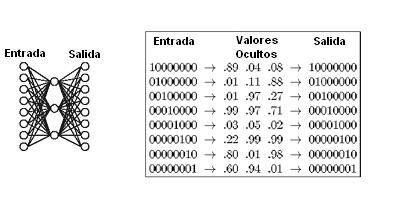
\includegraphics[scale=0.4,bb=0 0 406 203]{red1.png}
  \caption{ Ejemplo esquem�tico de una ANN.}
\end{figure}

\bigskip 
Dicho esto la elecci�n de una red neuronal como medio de resoluci�n del problema de reconocimiento de patrones ser�a en este caso la m�s acertada. Es muy �til cuando no se conoce la funci�n objetivo y se estima que los datos de entrada llegan con cierto porcentaje de ruido. La decisi�n se tom� meses antes de empezar el proyecto. Para asegurarnos de que era viable implementamos la red dentro de un peque�o programa, que a partir de im�genes de entrada devolv�a cierto si detectaba una imagen de una persona con una guante blanco y falso si no hab�a guante.

\section{Descripci�n t�cnica}
Hemos utilizado una red multicapa, ya que permiten representar superficies de decisi�n no lineales. Debido a esto no se puede utilizar unidades lineales ya que solo permitir�an representar funciones lineales. Tampoco pudimos utilizar perceptrones porque su funci�n de salida es discontinua, no derivable y por lo tanto no se le puede aplicar el descenso del gradiente. Necesit�bamos una unidad que diese como salida una funci�n no lineal y que fuese derivable con respecto a las entradas.

\bigskip 
Por eso utilizamos el sigmoide como unidad.

\begin{figure}[h]
  \centering
  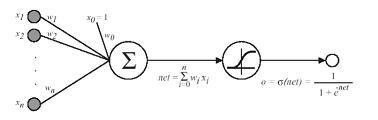
\includegraphics[scale=0.5,bb=0 0 378 120]{red2.png}
  \caption{ Unidad Sigmoide.}
\end{figure}

La funci�n sigma  $ \sigma(x)  = \frac{1}{(1+e^{-x})} $ es no lineal y derivable $ \frac{d\sigma(x)}{dx} =  \sigma(x) . (1 - \sigma(x)) $.

El descenso de gradiente se puede utilizar para entrenar:
\begin{itemize}
\item Una unidad sigmoide.
\item Una red multicapa de unidades sigmoides. Retropropagaci�n.
\end{itemize} 

La retropropagaci�n permite aprender los pesos para una red multicapa con un numero de unidades e interconexiones dado. Consideramos una red con m�ltiples unidades de salida, de forma que el error es la suma de los errores sobre todas las salidas. El espacio de hip�tesis viene dado por los valores posibles para los pesos de todas las unidades de red. Utilizamos el descenso de gradiente para encontrar una hip�tesis que minimice el error, el descenso utilizado es incremental, es decir, los pesos se actualizan despu�s de considerar cada ejemplo de entrenamiento en lugar de esperar a considerarlos todos. Es mas improbable que el descenso incremental caiga en un m�nimo local.
\bigskip 

La secuencia de pasos utilizada en nuestro entrenamiento viene a ser esta:
\begin{itemize}
\item Crear la red. 
\item Se inicializan los pesos de la red con valores peque�os y aleatorios entre -0.05 y 0.05
\item Para una media de 30 iteraciones se realiza lo siguiente: De una lista de im�genes de entrenamiento se va cogiendo una a una y se cargan en la capa de entrada de la red, para esa imagen se calculan las capas, luego seg�n un objetivo se calculo el error cometido en la capa oculta y en la salida y respecto a estos errores se reajustan los pesos de las interconexiones.
\item Se realiza un prueba y una validaci�n con im�genes distintas a las del entrenamiento, para ver el porcentaje de error total cometido, si es aceptable se guarda en un archivo los pesos de la red entrenada, para que en la fase de reconocimiento de im�genes solo haya que realizar el calculo de capas.
\end{itemize} 	

Para cada unidad de salida k, se calcula su termino de error: $ \delta_{k} = O_{k} . (1 - O_{k}) . (t_{k} - O_{k}) $

Para cada unidad oculta h, se calcula su termino de error: $ \delta_{h} = O_{h} . (1 - O_{h}) . \Sigma (W_{kh} . \delta_{k}) $ , siendo k las salidas.

Se actualiza cada peso de la red $ W_{ji} = W_{ji} + \Delta (W_{ji}) $ donde $ \Delta (w_{ji}) = \eta .\delta_{j} .x_{ji} + \alpha .\Delta w_{ji}. (n-1) $. 

($ t_{k} $ es la salida dada por ejemplo de entrenamiento para la unidad k. $ o_{t} $ es la salida generada por la red.)

La actualizaci�n de los pesos en la iteraci�n n depende de la actualizaci�n en n-1. El 2� termino de la ecuaci�n representa la cantidad de movimiento. Un s�mil f�sico seria una pelota que cae por la superficie de error, la cantidad de movimiento hace que la pelota tienda a mantener la misma direcci�n, con esto se intenta evitar que la pelota pare en un m�nimo local o que se pare en un llano.

\bigskip 
Respecto el descenso del gradiente en el sigmoide:
Para el descenso incremental consideramos el cambio en los pesos inducido por cada ejemplo de entrenamiento $ \Delta w_{ji} = \eta \frac{\eta E_{d}}{\eta w_{ji}} $ donde el error sobre un ejemplo de entrenamiento viene dado por la suma de los errores en cada unidad de salida $ E_{d}(w) \equiv \frac{1}{2} . \Sigma (t_{k} - o_{k})^{2} $ , siendo k las salidas

La salida viene dada por $ net = \Sigma w_{i}.x_{i} $ , i=0..n y $ o = \sigma (net) = \frac{1}{1 + e^{-net}} $, aplicando la regla de la cadena $ \frac{\eta E_{d}}{\eta w_{ji}} = \frac{\eta E_{d}}{\eta net_{j}} . \frac{\eta net_{j}}{\eta w_{ji}} = \frac{\eta E_{d}}{\eta net_{j}} . x_{ji} $. Para calcular $ \frac{\eta E_{d}}{\eta net_{j}} $ distinguimos el caso de las unidades de salida y las ocultas.

Error en las unidades de salida $ \frac{\eta E_{d}}{\eta net_{j}} = -(t_{j} - o_{j}). o_{j} .(1 - o_{j}) $. Error en la unidades ocultas $ \frac{\eta E_{d}}{\eta net_{j}} = o_{j} . (1 - o_{j}) . \Sigma (-\delta_{k} . w_{kj})  $.

\bigskip 
Para valores peque�os de los pesos (al principio del proceso) la red presenta una funci�n casi lineal donde es menos probable encontrar m�nimos locales. Cuando la funci�n es mas compleja (un punto mas avanzado del proceso) es de esperar que nos hayamos acercado tanto al m�nimo global que los m�nimo locales sean aceptables. Para garantizar que alcanzamos el m�nimo global utilizamos heur�sticas:
\begin{itemize}
\item A�adiendo cantidad de movimiento.
\item Utilizando descenso incremental.
\item Entrenar distintas redes con los mismos ejemplos, pero con distintos valores iniciales en los pesos.
\end{itemize} 

La capacidad expresiva de este tipo de red es bastante alta ya que:
\begin{itemize}
\item Cualquier funci�n booleana se puede representar con una red de dos capas.
\item Cualquier funci�n continua se puede aproximar con un error arbitrariamente peque�o por una red de dos capas.
\item Cualquier funci�n se puede aproximar con un error arbitrariamente peque�o por una red de tres capas (las dos ocultas de sigmoides y la de salida de unidades lineales).
\end{itemize} 

\section{Dise�o}
Esta formada por una capa de entrada, una de salida y una sola capa oculta.
Si imagin�semos la red como una caja negra, esta tendr�a que recibir como entrada una imagen y sacar como salida una cadena de texto explicativa de alg�n atributo de esa imagen.

\bigskip 
En nuestro caso la entrada ser�n siempre im�genes del mismo tama�o 320x240 p�xeles, por ello la capa de entrada consta de 76800 unidades. En realidad la entrada es un unsigned char* que representa la imagen con valores de 255 o 0, es decir, blanco o negro, recuerdo que las im�genes que le llegan a la red son im�genes que previamente han pasado por el modulo de filtro a si que llegan ya binarizadas. Estas entradas ser�n normalizadas entre 1 y 0, para que las entradas est�n en el mismo rango que las unidades de la capa oculta y de salida.

\bigskip 
La capa oculta debe tener tan pocas unidades como sea posible. Medidas experimentales demuestran que el hecho de aumentar el n�mero de  unidades ocultas proporciona mejoras poco significativas en la precisi�n, pero requieren mucho mas tiempo de entrenamiento. Nosotros hemos optado por utilizar 15 unidades.

\bigskip 
Como ya sabemos al robot se le controla con 2 manos, los gestos de la mano izquierda le indican las ordenes y los de las derecha los par�metros, con el objetivo de simplificar el dise�o los gestos de ordenes y de par�metros son los mismos, pero significan cosas distintas. Tanto para ordenes como para par�metros hay 5 tipos de gestos. Como recordatorio las ordenes eran: parar, avanzar, girar a la izquierda y girar a la derecha. Y los par�metros eran nula, medio baja, medio alta, alta si la orden actual es la de avanzar, donde los par�metros indican la velocidad a la que debe hacerlo o 0�, 45�, 90�, 180� si la orden actual es una de giro. La 5� gesto tanto para ordenes como para par�metros es el ``gesto no reconocido''. Por tanto dado que hay 5 tipos de gestos ha reconocer, la red tendr� que sacar 5 posibles salidas. Al principio optamos por una capa de salida de una sola unidad. El valor oscila entre 0 y 1 as� que por ejemplo si esta unidad val�a 0.2 significaba que hab�a reconocido el 2� gesto, si val�a 0.8 hab�a reconocido el 4� gesto. Luego se cambio al dise�o actual que es una capa de salida de 5 unidades, esto hace a la red mucho mas fiable, se pod�a decir que la salida de la red antes era anal�gica y ahora es digital, ya que todas las salidas tendr�n valores menores de 0.5 excepto una que ser� mayor, solo hay que asociar la unidad de la salida que se ha puesto en alta con una cadena de texto. Esta asociaci�n se hace mediante un script en Lua, as� es m�s modificable ya que si se quiere cambiar el texto de salida no hay que recompilar el proyecto, solo cambiar un archivo de texto.

\bigskip 
La organizaci�n de red por capas es est�ndar, la salida de cada unidad alimenta a todas las unidades de la siguiente capa.

La tasa de aprendizaje utilizada ha sido 0.3. La mas alta posible para reducir el tiempo de aprendizaje sin disminuir la precisi�n.

El descenso de gradiente es incremental para reducir el riesgo de quedarnos en m�nimos locales.

Los pesos de la unidades de salida y oculta son inicializados con peque�os valores aleatorios entre 0.05 y -0.05.

\section{Entrenamiento}
La mayor parte del c�digo utilizado en la red esta dirigido al entrenamiento. Por eso decidimos hacer un programa aparte que contiene el c�digo de entrenamiento de la red y luego el c�digo que est� presente en el proyecto que solo contiene el necesario para crear una red, calcular los valores de las capas a partir del valor de la capa de entrada y generar la cadena de texto de salida. As� el c�digo del proyecto queda mas sencillo para leer.

\bigskip 
El proceso de entrenamiento empieza con la sesi�n fotogr�fica, es necesario hacer mas de un centenar de fotos para obtener un entrenamiento medianamente fiable. Nosotros para el entrenamiento de ordenes sacamos 185 fotos, consiste en sacar fotos d�ndole ordenes al robot correctas, err�neas o simplemente no d�ndoselas. Todas estas fotos han de ser filtradas del mismo modo que lo har�a el modulo de filtro del proyecto, la raz�n de hacer un filtrado previo es poder pasar a la red im�genes muy simples, tambi�n deben de ser tomadas en unas condiciones de iluminaci�n similares a las que tendr� el entorno por el que circule el robot. No es lo mismo hacer aprender a la red a reconocer un gesto perdido en un mar de p�xeles de miles de colores a reconocer un conjunto de p�xeles blancos centrados sobre un fondo negro. Los objetivos mas perseguidos en este proyecto es la eficiencia y en este caso la fiabilidad en el reconocimiento.

\bigskip 
Las fotos son nombradas con un formato determinado, por ejemplo, ``\_orden\_parada\_21.bmp'' esto significa que la foto contiene la orden de parada y ``\_no\_gesto\_51.bmp'' indica que la foto no representa ninguna orden para el robot. Este formato es utilizado en el entrenamiento para que la red sepa ir reajustando los pesos seg�n el nombre explicativo de la foto.

\begin{figure}[h]
  \centering
  \includegraphics[scale=0.5,bb=0 0 160 120]{_no_gesto_36.png}
  \caption{ \_no\_gesto\_36.png}
\end{figure}

Todas las fotos no son utilizadas para el entrenamiento. Se hacen 3 listas de fotos que se utilizaran para el entrenamiento, la prueba y la validaci�n. Estas 2 ultimas sirven  para comprobar el buen funcionamiento de la red entrenada.

El objetivo del programa de entrenamiento es crear una red, entrenarla y salvar la estructura y pesos de red en un archivo.

El entrenamiento consiste en :
\begin{itemize}
\item Recorrer la lista de im�genes de entrenamiento una por una.
\item Cargar la imagen en la imagen en la capa de entrada, cada valor de p�xel se asocia a una unidad de la capa.
\item Seg�n el nombre de la foto, ejemplo ``\_orden\_parada\_21.bmp'', se cambia el objetivo, esto sirve para calcular el error cometido.
\item Cambiado el objetivo, se calcula el valor de la capas respecto a la capa de entrada, se calcula el error cometido en las capas oculta y salida y se reajustan los pesos, para disminuir el error.
\item Esta lista es recorrida un numero finito de iteraciones. Las condiciones de parada pueden ser varias. La nuestra es simplemente un numero concreto, en este caso fueron 30 iteraciones. Por tanto los pesos fueron ajustados 30x(numero de fotos de la lista) veces.
\end{itemize}
Ya tendr�amos as� unos pesos que representan una aproximaci�n a la funci�n buscada.
\bigskip 

\begin{figure}[h]
  \centering
  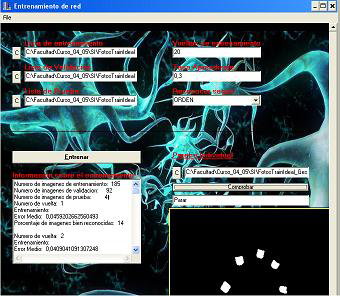
\includegraphics[scale=0.4,bb=0 0 340 296]{prog_train.png}
  \caption{ Captura de nuestro programa de entrenamiento de redes.}
\end{figure}

\bigskip 
Estos fueron datos de un entrenamiento de la red:
\begin{itemize}
\item Datos entrada:
\begin{itemize}
\item 148 fotos de entrenamiento, 49 fotos de validaci�n y 30 de prueba.
\item �ndice de aprendizaje: 0.3
\item 20 iteraciones
\end{itemize} 
\item Datos salida:
\begin{itemize}
\item Porcentaje de aciertos en entrenamiento: 89   Error medio: 0,0141046521582562
\item Porcentaje de aciertos en validaci�n: 93    Error medio: 0,00799933215976971
\item Porcentaje de aciertos en prueba: 100     Error medio: 0,00645778571591585
\end{itemize} 
\end{itemize}   

\begin{figure}[h]
  \centering
  \includegraphics[scale=0.4,bb=0 0 504 231]{Grafica_Aciertos.png}
  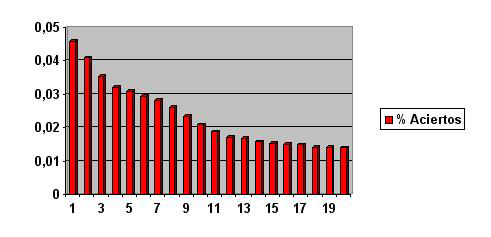
\includegraphics[scale=0.4,bb=0 0 491 237]{Grafica_Errores.png}
  \caption{ La imagen de la izquierda muestra como aumenta el aprendizaje cuanto mas se ense�a a la red. Aumentando el n� de aciertos. Y la de la derecha muestra como a medida que aprende comete menos errores reconociendo figuras.}
\end{figure}

\section{Red Neuronal en el proyecto}
Como cada modulo del pipeline, el modulo de red tiene un peque�o numero de funciones fijas utilizadas para ser llamadas desde el pipeline. Tres de ellas son ``red\_iniciar'', ``red\_cerrar'' y ``red\_ciclo''. Iniciar crea la red y carga el archivo creado por el programa de entrenamiento, por ejemplo el ``orden\_net''. La funci�n cerrar libera toda la memoria. Y la funci�n ciclo lo �nico que hace es recibir un char* que representa la imagen, cargar estos valores normalizados en la capa de entrada y calcular el valor de las capas oculta y de salida seg�n los pesos, que solamente tarda aproximadamente 0.10 segundos. Luego como ya dijimos solamente una de las cinco unidades de la capa de salida tendr� un valor superior a 0.5, esto es equivalente a que se ha puesto en ALTA y el modulo sacar� como salida la cadena de texto asociada a esa unidad. Cadena modificable desde un script junto con el nombre del archivo de la red entrenada. Todo lo que sea modificable en un futuro por posibles mejoras son par�metros que van escritos en scripts.

\bigskip 
Estas son 5 im�genes filtradas de ejemplo, cada una representa una orden o un par�metro.

Recordatorio:
\begin{itemize}
\item 1 dedo: Orden: Avanzar, Par�metro:  Medio baja o 45�
\item 2 dedos: Orden: Girar derecha,  Par�metro:  Medio alta o 90�
\item 3 dedos: Orden: Girar Izquierda,  Par�metro:  Alta o 180�
\item  5 dedos: Orden: Parar ,  Par�metro:  Nula o 0�
\end{itemize} 
 
\begin{figure}[h]
  \centering
  \includegraphics[scale=0.4,bb=0 0 160 120]{_orden_parada_17.png}
  
\includegraphics[scale=0.4,bb=0 0 160 120]{_orden_avanza_38.png}
  
\includegraphics[scale=0.4,bb=0 0 160 120]{_orden_angulo_43.png}
  \includegraphics[scale=0.4,bb=0 0 160 120]{_orden_negAngulo_84.png}
  \caption{ Ejemplos de imagenes de entrada en la red.}
\end{figure}

\section{Evoluci�n}
El primer sistema utilizado para resolver el problema de reconocimiento de gestos, fue la implementaci�n de dos redes distintas una para ordenes y otra para par�metros, debido a que su estructura era distinta.

Se fueron modificando los filtros con el objetivo de facilitar el aprendizaje a la red.

La segunda elecci�n fue utilizar el mismo numero de gestos tanto en ordenes como en par�metros as� se pudo conseguir la misma implementaci�n para ambas.

Luego se redujo considerablemente el c�digo, eliminando la parte de entrenamiento del proyecto. El c�digo de entrenamiento pasar�a a ser un programa a parte que generar� archivos de redes entrenadas. En este punto hab�a 2 archivos uno para cada red.

Y por ultimo visto que los gestos de las ordenes eran reconocidos con mucha mas facilidad que los asignados a los par�metros, que fallaban constantemente, decidimos que los gestos de los par�metros fuesen iguales a los de las ordenes, solo que en vez de hacer gestos con la izquierda se hacen con la derecha. De esta manera ambas redes cargan el mismo archivo y son igual de fiables. Solo se diferencian por la cadena de texto que devuelven, pero eso va por scripts.

\section{C�digo}
Ver anexo: documentaci�n del m�dulo de red.c y red\_neuronal.c, en \ref {red_code} (p�gina \pageref{red_code}).



\end{document}
